\chapter{Introduction}
\label{chap:introduction}
This is a citation: \cite{Vaswani2017}


This is a figure: 

\begin{figure}[ht]
    \centering
    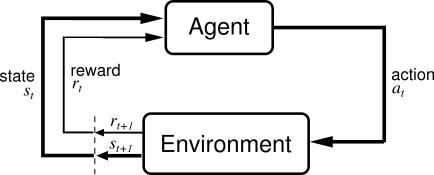
\includegraphics[width=.5\textwidth]{figures/AgentEnviornment.png}
    \caption{I am a caption}
    \label{fig:my_label}
\end{figure}



\section{Begin Intro}
In recent years, image anomaly detection has become significantly more important among many scientific communities, especially in industrial applications. This is no surprise, considering the
amount of mechanically manufactured parts in factories all over the world. Since in most parts of the world, manufactured items undergo more or less strict regulations and are expected to work
in real case scenarios, there is a need for sufficient quality control, that is rising with the amount of produced components. A long time ago, it has come to a point where human based quality 
checks are not adequate anymore for the production volume, which has led to computer solutions for the problem. Generally speaking, anomaly detection has first been proposed in 1986 for 
intrusion detection systems. While the methods and modalities may change, the high level idea stays the same: Detecting data that deviates from a set standard to a degree that is becoming
problematatic regarding the own requirements(letzer part maybe neu formulieren). Besides many approaches that were used over the years, deep learning approaches for image anomaly detection have
become very popular lately. A likely reason for this are impressively high performance scores with state of the art models achieving an area under the receiver operateor curve of around 0.96 and 
sometimes even more.
It is difficult to say what the first deep learning approaches to this topic were(dact checking), but a notable milestone is definetly Bergmann 2021(Referenz). Among blabla, they introduced
the MVTecAD dataset which is used widely and serves as a dataset to benchmark on for nearly every IAD paper released afterwards.






\section{Contributions}
This work builds upon the researched anomaly detection methods that were established as state of the art over the last years. paper1 and paper2 provide extensive overviews of all SOTA methods,
including the ones mentioned here. The main contributions thus are:
1. Creating a pipeline for anomaly detection experiments and inference, utilizing existing IAD approaches. 
2. Introducing three new categories for the mvtec(LOCO) dataset for anomaly detection experiments.
3. Researching anomaly detection performance on multi perspective datasets.
4. Experiment on the usage of different ensemble methods for IAD, including utilizing neural networks to learn proper ensemble weights.

The above contributions can be used as basis for industrial usage, aswell as a basis for future contributions on ensemble methods in the IAD space. Moreover it gives further insight on the
efficiency of SOTA IAD methods on different kinds of data than the previous synthetic settings.



-- in my work i contribute the following things:
- pipeline to infer new images on different algorithms and compare them
-> pipeline is industry focussed for benefits of the guys where i write my thesis

- research on multi perspective detection

- research of ensemble output learning to enhance individual network performance
-> simple network over 5-6 outputs

- introduction of very new dataset categories in style of mvtec LOCO dataset

